\documentclass{article}
\usepackage{ctex,soul,float,listings,enumerate,hyperref,url,amsfonts,amsmath,graphicx,multirow}
\usepackage{xcolor,tocloft,theorem,numerica,amsmath,mathrsfs}
\usepackage{changes}
\usepackage{fancyhdr}
%%%%%%%%%%%%%%%%%%%%%%%%
\definecolor{AnatationColor}{RGB}{0,139,0}
\lstset{
    backgroundcolor = \color{white},    % 背景色:白色
    basicstyle = \small\ttfamily,           % 基本样式 + 小号字体
    rulesepcolor= \color{white},             % 代码块边框颜色,白色
    breaklines = true,                  % 代码过长则换行
    numbers = left,                     % 行号在左侧显示
    numberstyle = \small,               % 行号字体
    keywordstyle = \color{blue},            % 关键字颜色
    commentstyle =\color{AnatationColor},        % 注释颜色
    stringstyle = \color{red!100},          % 字符串颜色
    frame = shadowbox,                  % 用(带影子效果)方框框住代码块
    showspaces = false,                 % 不显示空格
    columns = fixed,                    % 字间距固定
    %escapeinside={<@}{@>}              % 特殊自定分隔符:<@可以自己加颜色@>
    morekeywords = {as},                % 自加新的关键字(必须前后都是空格)
    deletendkeywords = {compile}        % 删除内定关键字;删除错误标记的关键字用deletekeywords删!
}
\hypersetup{
    colorlinks=true,
    linkcolor=red,
    filecolor=blue,      
    urlcolor=blue,
    citecolor=cyan,
}
\newtheorem{definition}{定义}
\graphicspath{{./Image/}}
%%%%%%%%%%%%%%%%%%%%%%%%
\author{ZeitHaum}
\date{\today}
\title{C++ 进阶用法}
\pagestyle{fancy}
%%%%%%%%%%%%%%%%%%%%%%%%
\begin{document}
    \pagenumbering{Roman}
    \maketitle
    \newpage 
    \tableofcontents
    \newpage
    \setcounter{page}{1}
    \pagenumbering{arabic}
    \section{C++ lambda表达式}
    C++ 11以上特性。

    \begin{figure}[H]
        \centering
        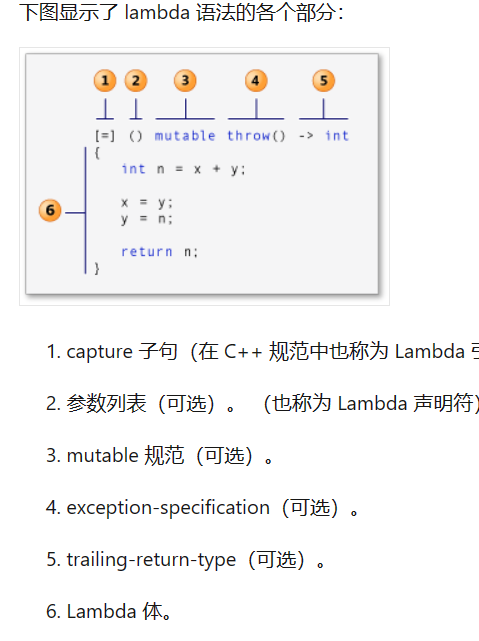
\includegraphics[width = 0.9\textwidth]{fig1.png}
    \end{figure}

    \subsection{capture子句}
    用于访问(捕获)外部变量。
    [=]用于值捕获,[\&]用于引用捕获,[this]捕获外部类指针this([\&]默认包含[this])。
    补充:[args...]用于捕获外部可变参数模板。
    \subsection{返回类型}
    编译器自动推导。也可以使用关键字``->''指定,此时不能省略空参数列表。

    \subsection{mutable}
    在按值捕获时无法在作用域内修改外部变量的值,使用mutable修饰后可以解决这个问题。但是修改仅限于lambda表达式内部生效。
    \lstinputlisting[language=c++]{TestCode1_1.cpp}
    输出结果为
    \begin{figure}[H]
        \centering
        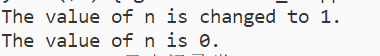
\includegraphics[width = 0.5\textwidth]{fig3.png}
    \end{figure}
    
    \section{迭代器}
    迭代器用于访问顺序容器(主要是vector和数组)。
    \subsection{分类}
    分为正向迭代器、常量正向迭代器、反向迭代器、常量反向迭代器。
    比较常用的是正向迭代器和反向迭代器,反向迭代器的开始和结束分别为rbegin()和rend()。

    二者区别在于正向迭代器++返回顺序容器后一个数,后者返回前一个数。
    以下是二者使用的一个例子:
    \lstinputlisting[language=c++]{TestCode2_1.cpp}
    
    输出结果为
    \begin{figure}[H]
        \centering
        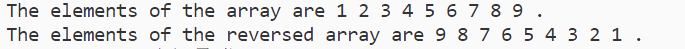
\includegraphics[width = 0.7\textwidth]{fig4.png}
    \end{figure}

    数组的迭代器就是指针,使用``数组名+N''的形式表示。

    \subsection{不同容器中的迭代器}
    根据容器类型的不同,可将迭代器分为正向迭代器、双向迭代器、随机访问迭代器,
    限制依次呈递减趋势。
    其中数组和vector的迭代器都是随机访问迭代器。
    其支持的功能如下:
    \begin{figure}[H]
        \centering
        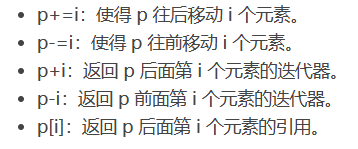
\includegraphics[width = 0.5\textwidth]{fig5.png}
    \end{figure}
    另外p2 - p1 和p1 < p2均有定义(和索引类似)。

    不同容器的迭代器类型如下:
    \begin{figure}[H]
        \centering
        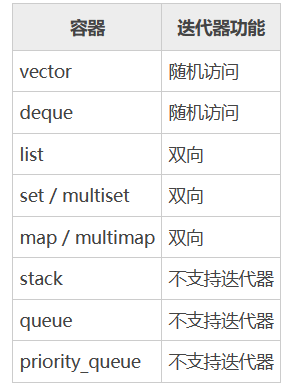
\includegraphics[width = 0.5\textwidth]{fig6.png}
    \end{figure}

    \subsection{辅助函数}
    C++ 中关于迭代器的辅助函数为advance、distance、iter\_swap;
    其功能如下:
    \begin{figure}[H]
        \centering
        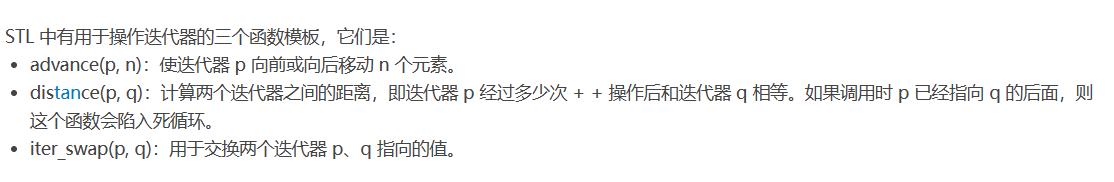
\includegraphics[width = 0.9\textwidth]{fig7.png}
    \end{figure}

    \section{algorithm库中常用函数}
    algorithm是C++ 标准库之一,需使用using namespace std;语句引入名称空间。
    
    algorithm库函数具有丰富的可扩展性,这些需要使用lambda表达式和迭代器实现。


    \subsection{all\_of}
    对列表中的元素执行谓词,如果都为真返回true.
    
    例子:
    \lstinputlisting[language=c++]{TestCode3_1.cpp}
    输出:
    \begin{figure}[H]
        \centering
        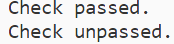
\includegraphics[width = 0.3\textwidth]{fig8.png}
    \end{figure}
    \subsection{any\_of}
    和all\_of区别是有任一为真即返回true.

    \subsection{none\_of}
    无一为真返回true.

    \subsection{for\_each}
    为每个函数执行操作,输入可以是函数指针也可以是lambda表达式。
    
    例子:
    \lstinputlisting[language=c++]{TestCode3_2.cpp}

    输出结果为
    \begin{figure}[H]
        \centering
        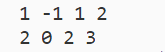
\includegraphics[width = 0.9\textwidth]{fig9.png}
    \end{figure}

    \subsection{generate}
    类似于for\_each,只是更新方式由参数指针修改变为返回值赋值。
    
    \subsection{generate\_n}
    类似于generate,只是结束迭代器被换为了大小n。(从开始迭代器开始,包含开始迭代器。)

    \subsection{includes}
    对于两个\textbf{已经排序好的(增序)}的范围[first1,last1) 和[first2,last2),检查对于[first2,last2)中的元素,
    是否\textbf{所有的}元素都被包含在[first1,last1)中。

    若[first1,last1)为空,C++98返回不确定值,而C++11返回真。

    例子:
    \lstinputlisting[language=c++]{TestCode3_3.cpp}

    输出结果为
    \begin{figure}[H]
        \centering
        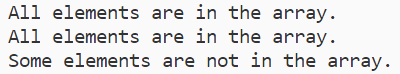
\includegraphics[width = 0.6\textwidth]{fig10.png}
    \end{figure}

    \subsection{inplace\_merge}
    合并两部分\textbf{已经排好序的}数组,不常用。

    \subsection{is\_heap}
    检查一个数组是否是一个堆。

    \subsection{is\_heap\_until}
    返回一个数组第一个不满足堆性质的非法字符。

    \subsection{is\_partitioned}
    若满足谓词性质的元素均在不满足谓词的元素前返回true,否则返回false.

    

    \section*{参考文献}
    \addcontentsline{toc}{section}{参考文献}
    [1]. \href{https://learn.microsoft.com/zh-cn/cpp/cpp/lambda-expressions-in-cpp?view=msvc-170}{Microsoft C++、C 和 汇编程序}
    
    [2]. \href{https://blog.nowcoder.net/n/91357602b82d4377917a35afde085ff8}{C++ algorithm 头文件下常用函数整理}

    [3]. \href{http://c.biancheng.net/view/338.html}{C++迭代器(STL迭代器)iterator详解}

    [4]. \href{https://cplusplus.com/reference/algorithm/}{cplusplus.com-algorithm}

\end{document}
